Afin d'ajouter une nouvelle table dans la base de données, il est nécessaire de modifier le fichier models.py présent dans le dossier tennis (Figure~\ref{}). Pour ce faire, il suffit d'ouvrir le fichier à l'aide d'un éditeur de code (Notepad, Pycharm, etc.), et de rajouter une nouvelle classe à la fin de celui-ci en respectant l'indentation et la syntaxe python appropriée. La structure d'une classe est définie sur la figure~\ref{fig:Structure d'une classe représentant une table de la base de données}

\begin{figure}[!ht]
\centering
\begin{framed}
\lstinputlisting[language=Python, firstline=1, lastline=8]{"developer_guide/class.py"}
\end{framed}
\caption{Structure d'une classe représentant une table de la base de données}
\label{fig:Structure d'une classe représentant une table de la base de données}
\end{figure}
\FloatBarrier

Cette structure se complète ensuite en définissant l'ensemble des variables de classe (représentant les différentes informations à stocker dans la base de données) en spécifiant leurs types et leurs éventuelles relations et en y complétant les méthodes \textit{str} et \textit{unicode}. On peut observer un exemple d'une telle classe sur la figure~\ref{fig:Classe issue du fichier models.py représentant une table de la base de données}

\begin{figure}[!ht]
\centering
\begin{framed}
\lstinputlisting[language=Python, firstline=9, lastline=24]{"developer_guide/class.py"}
\end{framed}
\caption{Classe issue du fichier \textit{models.py} représentant une table de la base de données}
\label{fig:Classe issue du fichier models.py représentant une table de la base de données}
\end{figure}
\FloatBarrier

Les types principaux sont les suivants :\\

\begin{itemize}
\item models.CharField : un champ contenant une chaine de caractères
\item models.AutoField : un champ contenant un entier se remplissant de manière automatique et incrémentale en fonction des identifiants disponibles
\item models.BooleanField : un champ contenant un booléen (vrai ou faux)
\item models.DecimalField : un champ contenant un nombre décimal de taille fixe
\item models.DateTimeField : un champ contenant un date et une heure
\item models.TextField : un champ contenant une chaine de caractère (de très grande taille)\\
\end{itemize}

A noter qu'il est également possible de spécifier divers options (à passer en paramètres lors de la création de la variable), tels que la taille maximale du champ, la valeur par défaut, si le champ est obligatoire où non, ...\\

Les relations principales sont les suivantes :\\
\begin{itemize}
\item models.ForeignKey : une relation plusieurs-à-un (one to many)
\item models.OneToOneField : une relation un-à-un
\item models.ManyToManyField : une relation plusieurs à plusieurs\\
\end{itemize}

Il est également possible de passer plusieurs options en paramètres lors de la création des relations, comme le nom à utiliser pour la relation inverse depuis l’objet lié vers celui-ci, si le champ est obligatoire ou non, ...\\

L'ensemble des types, relations et options sont consultables dans la documentation Django à l'adresse suivante : https://docs.djangoproject.com/fr/1.9/ref/models/fields/.\\

Une fois l'ensemble des variables définies, il est également possible de définir certaines fonctions de classe, avec la syntaxe def nomDeFonction (self) : . Cela peut s'avérer utile pour retourner certains champs en particulier, ou certaines combinaisons de champs en les concaténant au préalable (adresse, informations personnelles, ...).\\

Une fois terminé, il ne reste qu'à sauvegarder les modifications apportées au fichier, le fermer, et effectuer la migration de la base de données (afin que ceux-ci soient bien effectués) grâce aux commandes (dans cet ordre) : python manage.py makemigrations et python manage.py migrate. Un nouveau fichier contenant les modifications apportées à la base de données sera créé dans le dossier ASMAE/tennis/migrations, ce qui permet d'avoir une vue d'ensemble de l'évolution de la base de données mais surtout de pouvoir effectuer des restaurations à des versions antérieures (rollbacks) si besoin est.\\

\begin{figure}[H]
\centering
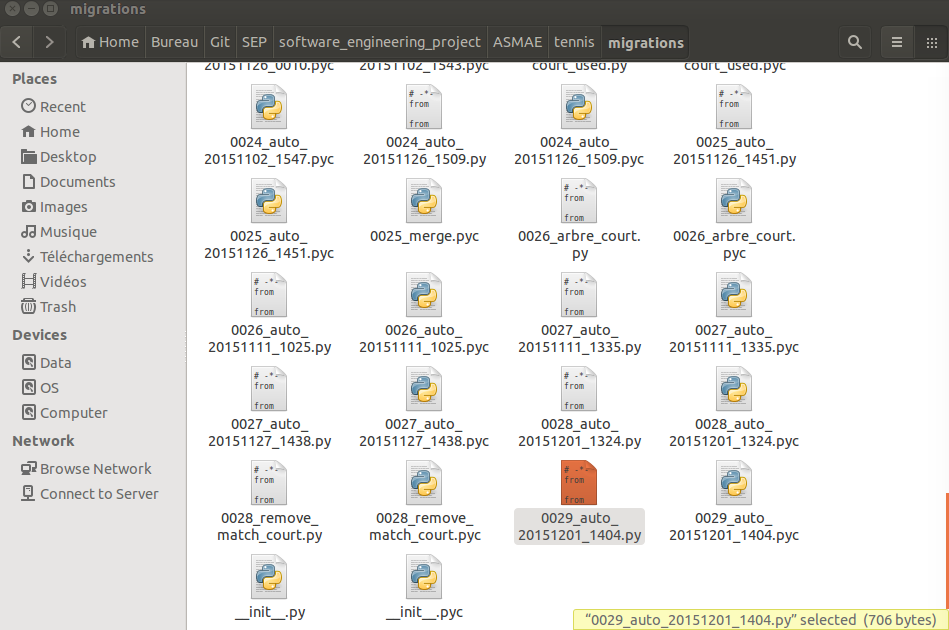
\includegraphics[scale=0.4]{Migration1.png}
\caption{Migration}
\end{figure}

\begin{figure}[H]
\centering
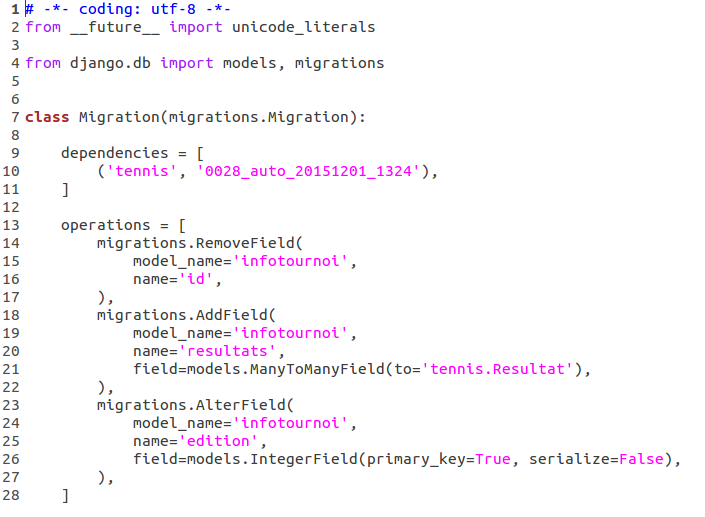
\includegraphics[scale=0.4]{Migration2.png}
\caption{Migration}
\end{figure}

L'ensemble de la documentation se rapportant aux commandes de migration de la base de données est disponible à l'adresse suivante : https://docs.djangoproject.com/en/1.9/topics/migrations/.\\

Une fois la migration effectuée, il est possible de directement aller vérifier sur la nouvelle table a correctement été ajoutée, ou si la ou les modifications ont bien été apportées à la base de données via l'interface administration de Django. Il suffit pour cela de se connecter à l'adresse du site web suivi de "/admin" avec les identifiants d'administrateur, et de se rendre dans l'onglet "Tennis".\\

\begin{figure}[H]
\centering
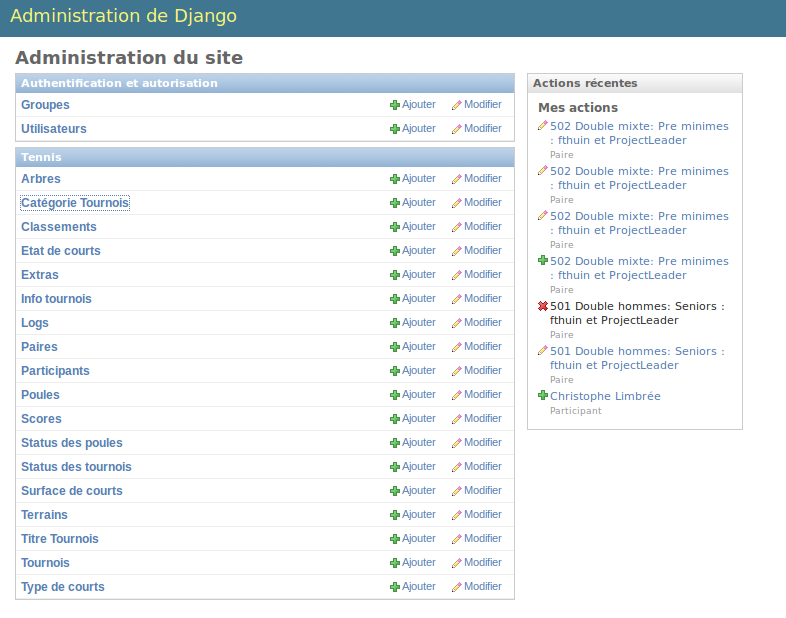
\includegraphics[scale=0.4]{Admin.png}
\caption{Interface administrateur}
\end{figure}

Il est intéressant de noter que la même démarche peut être suivie lorsqu'une ou plusieurs modifications doivent être apportées à une table déjà existante dans la base de données.\\

Ajouter une view et template correspondant :\\

Afin de rajouter du nouveau contenu sur le site internet, il est utile de pouvoir créer de nouvelles pages, et de les rendre accessibles à partir de celles déjà présentes.\\

Pour ce faire, il faut dans un premier temps créer le template, c'est à dire la structure de la page en HTML. Une fois le fichier représentant la page créé, il faut l'ajouter au dossier contenant l'ensemble des pages HTML du site, c'est-à-dire "ASMAE/tennis/templates". Il est intéressant de noter que les différents éléments statiques (tels qu'un style css, police particulière, ...) doivent être ajoutés dans le sous-dossier correspondant, présent dans le répertoire "ASMAE/tennis/static/tennis".\\

\begin{figure}[H]
\centering
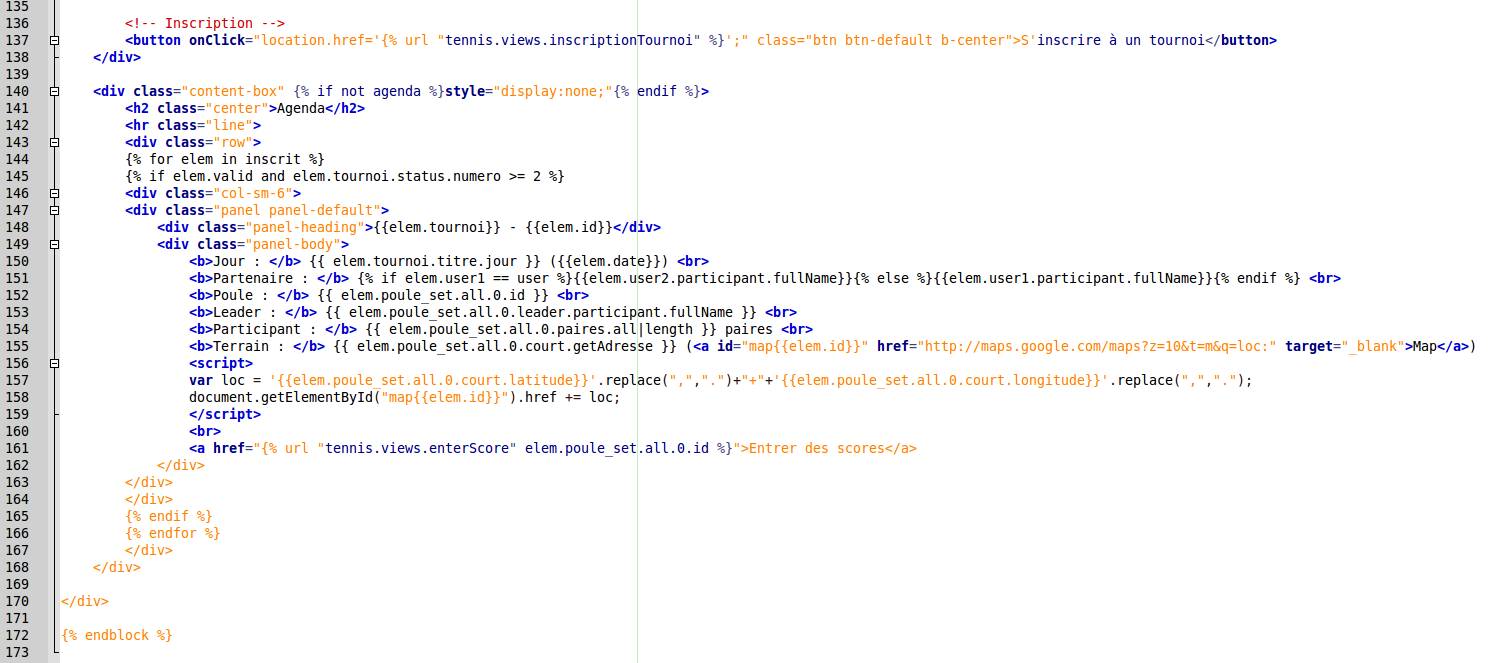
\includegraphics[scale=0.3]{html.png}
\caption{Exemple d'une page HTML}
\end{figure}

Une fois fait, il est nécessaire de créer une view dans le fichier views.py se trouvant dans le dossier "ASMAE/tennis", qui reprendra la page à renvoyer quand un utilisateur fera une requête pour obtenir la page. Le format le plus classique et simpliste d'une telle requête est le suivant: on définit le nom de la requête, ainsi que la page à rendre quand celle-ci est effectuée.\\

\begin{figure}[H]
\centering
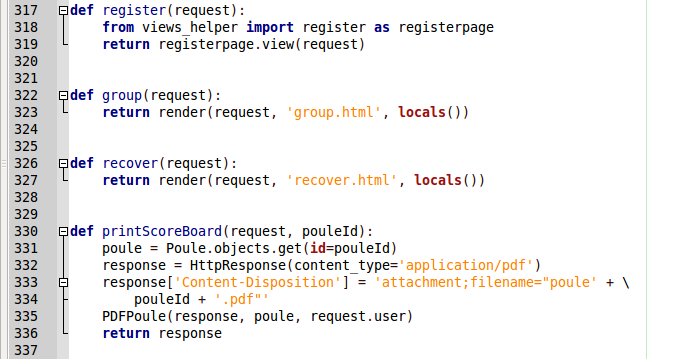
\includegraphics[scale=0.4]{views.png}
\caption{Fichier views.py}
\end{figure}

Enfin, il reste à ajouter au fichier urls.py (également présent dans le dossier "ASMAE/tennis") qui contient tous les liens URL disponibles sur le site, ainsi que le lien vers le nom des views concernées. Pour ce faire, il suffit de rajouter une nouvelle ligne dans le fichier, en respectant le format suivant : url(NouveauLienUrl, NomDeLaViews), .

\begin{figure}[H]
\centering
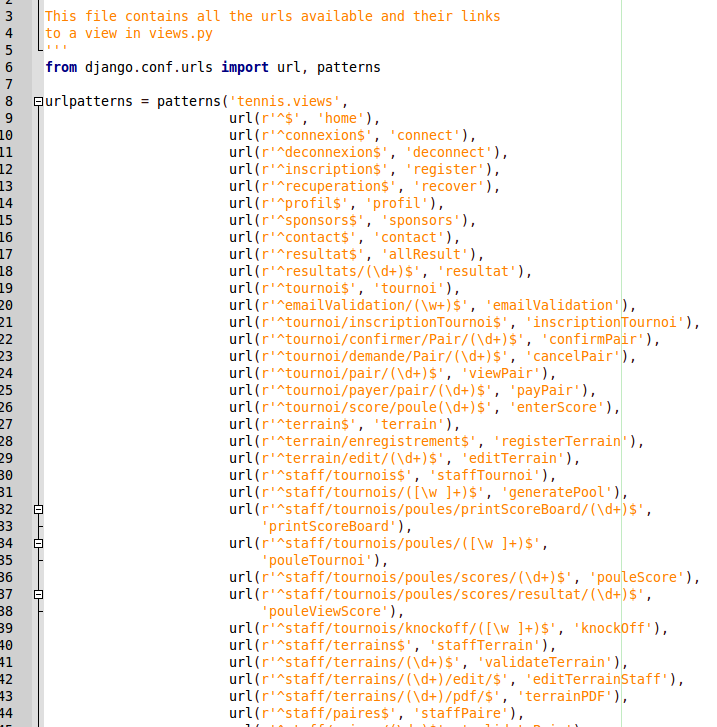
\includegraphics[scale=0.4]{url.png}
\caption{Fichier urls.py}
\end{figure}
